\documentclass[a4paper,12pt]{article}
%For images
\usepackage{graphicx}
 
\addtolength{\oddsidemargin}{-.875in}
\addtolength{\evensidemargin}{-.875in}
\addtolength{\textwidth}{1.75in}
 
\addtolength{\topmargin}{-.875in}
\addtolength{\textheight}{1.75in}
 
\begin{document}
\begin{enumerate}
      \item Enligt Faraday's lag är volten $e=Bvl$ med v som hastigheten
            l=1.2 som längden på kofångaren och B=0.050 som gjordens magnetfält,
            fast man multiplicerar med sinus av inklinationsvinkeln då
            man vill ha fram det som påverkar kofångaren.
            Volten för ledlampor är ungefär 1.5 V. Då blir det

            $$v=\frac{e}{\sin(\theta)Bl}=\frac{1.5}{\sin(71)0.050\cdot 1.2}=26.4m/s=95.1km/h$$

            Figuren nedan visar vad som händer, där den gråa linjen är kofångaren
            och de svarta pilarna är jordens magnetfält. Varför sin krävs blir nu självklart.
            \begin{center}
                  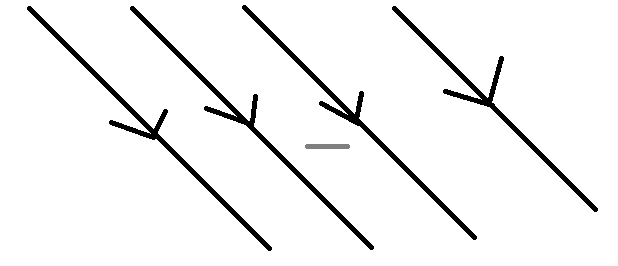
\includegraphics[scale=0.3]{figur1.png}
            \end{center}

      \item Med hjälp av "bil-regeln" så får man fram att
            svaret blir $F=BIL=0.10\cdot 3.5\cdot 0.08=0.028$N.

      \item
            \begin{enumerate}
                  \item Man beräknar ut effektivvärdet genom att
                        ta amplituden av ekvationen som beskriver dess värde över
                        tid och dividerar sedan den på roten ur två.
                        $$U=\frac{\hat{u}}{\sqrt{2}}=\frac{25.0}{\sqrt{2}}\approx 17.7V$$

                  \item Både Ohms lag och Joules lag håller i dom här sambanden.
                        Från förra uppgiften vet vi att $$U=\frac{\hat{u}}{\sqrt{2}}$$
                        Med Ohms lag får vi att $$I=\frac{U}{R}=\frac{\hat{u}}{R\sqrt{2}}$$
                        Och med Joules lag $$P=IU=\frac{\hat{u}^2}{2R}$$

                        Effekten blir då

                        $$\frac{25.0^2}{2\cdot 10}=31.25W$$

                        Eftersom att enheterna för effekten är i Watts vilket är Joules per sekund,
                        och eftersom uppgiften frågar efter energin som mäts i Joules så
                        multipliceras svaret med 60 och vi får att svaret blir $31.25\cdot 60=1 875$ Joules av energi.
            \end{enumerate}

      \item Från Ohms lag så blir $I=\frac{P_1}{U_1}$. För glödlampan i det gammla utaget.
            Men när det sätts in i det nya så blir effekten $P_2=IU_2=\frac{P_1}{U_1}U_2$ om man
            antar att strömmen bör vara konstant.
            Vilket skulle innebära att effekten skulle bli väldigt mycket högre än den annars klarar
            av. Runt 70 Watt istället för det vanliga 40 man får från uppgiften. Den skulle lysa
            väldigt starkt och gå sönder.

      \item
            \begin{enumerate}
                  \item
                        Vid transformatorer så är volten direkt proportionell till antalet varv.
                        Då blir det $$\frac{U_1}{U_2}=\frac{N_1}{N_2}\Rightarrow N_1=\frac{U_1N_2}{U_2}$$

                        Eftersom att $N_1$ är antalet varv på spolen som uppgiften frågar efter.
                        Då blir det
                        $$\frac{230\cdot 20}{4}=1150$$

                        Så svaret blir 1150 varv.
                  \item Effekten är konstant så då får vi att $$P=I_1U_1=I_2U_2\Rightarrow I_1=\frac{I_2U_2}{U_1}$$
                        $$=0.20\cdot 4 / 230 \approx 0.0035A=3.5mA$$
            \end{enumerate}

      \item Om vi säger att distansen mellan den första och andra ledaren är $r_1$ och
            den mellan andra och tredje är $r_2$, samt att vi numbrerar varje ledare
            med 1,2,3 från högst till lägst. Vi får då ut en kraftformula som utförs
            av ledare $I_1$ mot $I_2$.
            $$F=k\frac{I_1I_2L}{r_1}$$
            Samt den som utförs av $I_3$ mot $I_2$, vilket är motsatt till den andra kraften
            $$F=-k\frac{I_3I_2L}{r_2}$$
            Men konstanten k och längden L som snart kommer visa sig vara oviktiga för att lösa uppgiften.
            Eftersom att krafter kan summeras samt att uppgiften vill att dem ska summera
            till noll får vi följande jämnlikhet
            $$0=k\frac{I_1I_2L}{r_1}-k\frac{I_3I_2L}{r_2}$$
            $$\Rightarrow\frac{I_1}{r_1}=\frac{I_3}{r_2}$$
            $$\Rightarrow I_1 = \frac{I_3r_1}{r_2}=\frac{3\cdot 0.05}{0.02}=7.5A$$

      \item
            Ekvationen för inducerad spänning på grund av flödesförändring är
            $$U=N\frac{d\phi}{dt}=NA\frac{dB}{dt}$$
            Löser ut antalet varv
            $$N=\frac{U}{A}\frac{dt}{dB}$$

            Varenda gång en magnet går igenom oket så går flödet från 0 till maximalt flöde
            halv vägs förbi, för att sedan bli lika och motsatt när den är påväg ut ur oket.
            Eftersom att frekvensen är 75 så blir då $$dt=T/2=1/2f=1/150$$

            Magnetflödet dB ändrar sig med 0.4 under den tiden, dvs $\frac{dB}{dt}=\frac{0.4}{1/150}=60$.

            Så då blir antalet varv och svaret $$N=\frac{3}{0.0002}\cdot\frac{1}{60}=250$$

      \item
            \begin{enumerate}
                  \item Med ekvationen för inducerad spänning $e=vlB=6\cdot 0.15\cdot 1.5=1.35$V.
            \end{enumerate}
\end{enumerate}
\end{document}